\documentclass[a4paper,12pt]{report}

\usepackage{alltt, fancyvrb, url}
\usepackage{graphicx}
\usepackage[utf8]{inputenc}
\usepackage{hyperref}

% Questo commentalo se vuoi scrivere in inglese.
\usepackage[italian]{babel}

\usepackage[italian]{cleveref}

\title{Relazione\break``Farming Simulator''}

\author{Linda Fabbri, \\ Federico Raffoni,\\ Simone Rega,\\ Giacomo Montali}
\date{20 Aprile 2021}


\begin{document}

\maketitle

\tableofcontents

\chapter{Analisi}


\section{Requisiti}


Il gruppo si pone come obiettivo quello di realizzare "Farming Simulator", un software a scopo ludico basato sul videogioco "Hay Day" \footnote{\url{https://supercell.com/en/games/hayday/}} sviluppato da Supercell.
Il progetto mira alla realizzazione di un ambiente agricolo in 2D, in cui il giocatore interagisce con le colture e gestisce le proprie finanze.
Lo scopo del gioco è arrivare all'apice della ricchezza, sbloccando tutti gli appezzamenti di terra e coltivando la maggior varietà di semi possibili.


\subsubsection{Requisiti funzionali}
\begin{itemize}
	\item Questa applicazione deve permettere al giocatore di muoversi all'interno della mappa di gioco evitando di salire su zone di mappa non calpestabili.
	\item Il personaggio ha la possibilità di coltivare piantagioni di grano, patate, pomodori, carote, alberi di ciliege e altri frutti.
	\item Nella mappa deve comparire una zona per l'allevamento degli animali, grazie ai quali si possono raccogliere latte, uova e altri derivati.
	\item Farming Simulator mette a disposizione un negozio in cui è possibile vedere il proprio inventario, vendere i prodotti agricoli raccolti in cambio di monete virtuali e comprare nuovi semi da coltivare.
	\item Per aumentare la difficoltà di gioco vengono messi a disposizione appezzamenti di terreno coltivabili inizialmente bloccati, che si possono sbloccare tramite l'utilizzo delle monete virtuali.
\end{itemize}


\subsubsection{Requisiti non funzionali}
\begin{itemize}
	\item Farming Simulator deve poter essere eseguito su dispositivi con schermi dotati di risoluzioni differenti.
	\item Il programma deve poter essere eseguito sia su Windows sia su sistemi operativi Unix
\end{itemize}

\hfill\break
\section{Analisi e modello del dominio}

In Farming Simulator il soggetto principale è il personaggio virtuale, il quale si muove all'interno di una mappa, composta da diversi tipologie di blocchi. 
%
All'interno della mappa possiamo trovare blocchi coltivabili (Field Block), blocchi non calpestabili dal personaggio (Wall), blocchi estetici(Water), il quale unico compito è quello di abbellire la mappa, blocchi che compongono la stalla in cui possono muoversi gli animali(Stall), ed infine blocchi "locked"(Unlockable Block), ovvero che inizialmente sono bloccati e possono essere sbloccati durante la partita in cambio di monete virtuali.

Il personaggio (Player), grazie all'inventario (Inventory), è in grado di mantenere risorse al suo interno. Tra le risorse collezionabili possiamo trovare: il cibo (Food) ottenuto dalla raccolta di coltivazioni o di animali oppure i semi (Seed).
Questi ultimi possono essere comprati nel negozio (Shop) del videogioco, dentro il quale è anche possibile vendere il cibo che si è raccolto.

Il personaggio può interaggire con blocchi e animali (Animals), in particolare può piantare e raccogliere i semi all'interno dei blocchi coltivabili (FieldBlock), sbloccare i blocchi non ancora accessibili (UnlockableBlock) e raccogliere i prodotti animali.

\begin{figure}[!htb]
\centerline{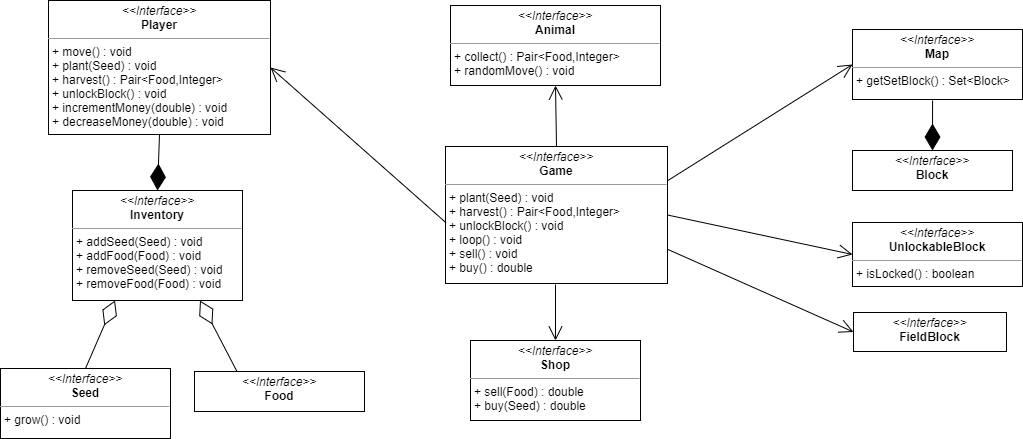
\includegraphics[scale=.7]{img/UML_1-1.png}}
\caption{Schema UML dell'analisi del problema, con rappresentate le entità principali ed i rapporti fra loro}
\label{img:analysis}
\end{figure}

\chapter{Design}

\section{Architettura}

L’architettura di Farming Simulator è basata su un pattern MVC. In particolare è stata sviluppata l’interfaccia Game che funge da Controller e si posiziona tra View e Model e gestisce eventuali interazioni tra componenti. All’arrivo di un input, game, si occupa di ordinare al Model il cambio di stato.

\hfill\break
Gli input da tastiera provenienti dall’utente passano attraverso la classe KeyNotifier, la quale si occupa di informare il game dell’avvenuto input. 

\hfill\break
La parte di View è formata da diversi GameDrawer, i quali si occupano di interrogare il game e mostrare a video il gioco.

Quando viene catturato un input da tastiera, il GameDrawer avvisa il keyNotifier dell’avvenuta pressione, così facendo il KeyNotifier è un observable per GameDrawer. In questo modo il GameDrawer non si deve occupare della gestione degli input, spostando il carico di lavoro al KeyNotifier; questa astrazione ci permette di non dipendere dall'implementazione e poter cambiare il binding\footnote[1]{Binding = associazione di un tasto ad un determinato movimento e/o interazione visiva in gioco (ad esempio [WASD] per spostarsi nella mappa)} o addirittura dispositivo di input (ad esempio un Joystick). 

\hfill\break
In \Cref{img:MVC} è esemplificato il diagramma UML che descrive l'architettura MVC del progetto, mostrando le classi principali.

\hfill\break
\begin{figure}[!htb]
\centerline{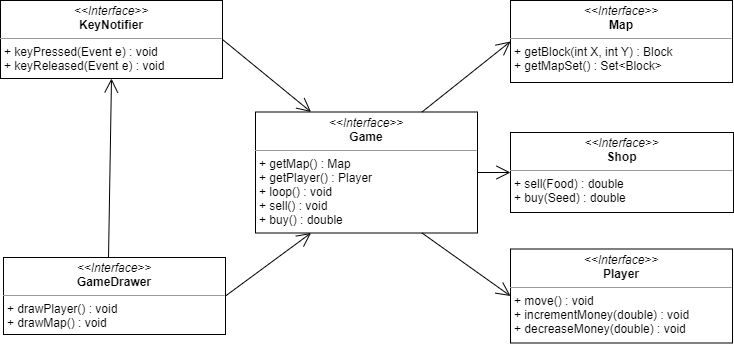
\includegraphics[scale=.65]{img/UML_2-1.png}}

\caption{Schema UML architetturale di Farming Simulator, MVC.}
\label{img:MVC}
\end{figure}





\section{Design dettagliato}

In questa sezione vengono mostrati alcuni elementi di design con maggior dettaglio.
Ogni membro del gruppo presenta gli elementi di design più significativi da lui prodotti, al fine di realizzare l’applicazione, predisponendola a future espansioni.



\subsection{Simone Rega}
Io nel progetto mi sono occupato della parte riguardante l’aggiornamento dinamico della GUI nella sezione dello Shop, in particolare mi preoccupo di aggiornare il JPanel dello shop e la visualizzazione dell’inventario ogni qualvolta che si interagisce con i JButton di compra/vendita, la JComboBox e il JSpinner per comprare semi. 

Ho ritenuto utile usare un pattern Observer in modo che al cambiamento di un osservatore, quindi un Evento sui componenti grafici descritti primi, gli altri osservatori vengono notificati per poi essere aggiornati.


È stato deciso insieme a\textit{ Federico Raffoni} di creare le interfacce \textbf{Observer} e \textbf{Observable} di tipo generico, in modo da poter implementare le classi in più possibili situazioni eterogenee.
Il ruolo di Observable è ricoperto dalla classe ObservableShopGUI mentre il ruolo di Observer è ricoperto da ObserverShop (classe innestata all’interno di ShopDrawer.java). 

\hfill\break
In \Cref{img:SimoneRega_Observer} è esemplificato il diagramma UML che descrive l'architettura del pattern Observer usato da Simone Rega, mostrando le classi principali.
\hfill\break

\begin{figure}[!htb]
	\centerline{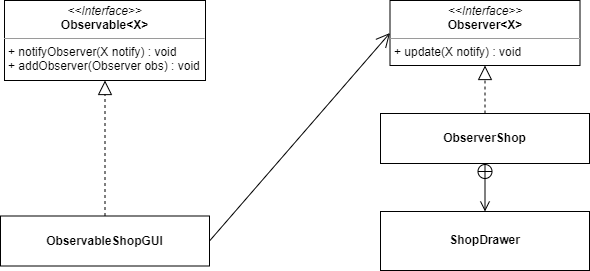
\includegraphics[scale=0.8]{img/UML_ObserverSimo.png}}
	
	\caption{Schema UML architetturale del pattern Observer (Simone Rega).}
	\label{img:SimoneRega_Observer}
\end{figure}

\subsection{Federico Raffoni}
In questa sezione ci occuperemo principalmente del caricamento delle risorse grafiche e non solo. In particolare è stata creata la classe Resources la quale si occupa di caricare e distribuire tutte le risorse. 

È stato usato il pattern SINGLETON per rendere unico nell’applicazione l’accesso alla classe Resources. In questo modo si evita che diversi GameDrawer carichino più volte le risorse sprecando memoria.

 Le risorse verranno caricate solo alla prima chiamata, mentre le chiamate successive riceveranno una copia statica della classe risparmiando tempo e risorse.
 
 In \Cref{img:FedericoRaffoni_Singleton} è esemplificato il diagramma UML che descrive l'architettura singleton, mostrando le classi principali.
\hfill\break

\begin{figure}[!htb]
	\centering{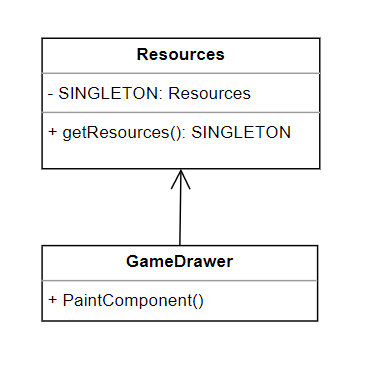
\includegraphics[scale=.6]{img/UML_SingletonRaffo.png}}
	\caption{Schema UML architetturale del pattern Singleton (Federico Raffoni).}
	\label{img:FedericoRaffoni_Singleton}
\end{figure}

Per quanto riguarda il caricamento di una partita salvata, è stato utilizzato il pattern Observer per consentire all’Engine di rimanere in attesa mentre la classe GamePreloader si occupa di chiedere alll’utente se continuare una partita salvata oppure iniziare una partita da zero.

In particolare Engine è Observer, mentre la classe GamePreloader è Observable.  Sono state realizzate inoltre le interfacce Observer e Observable generiche, in modo da poter essere riutilizzate anche in altri campi.

 In \Cref{img:FedericoRaffoni_Observer} è esemplificato il diagramma UML che descrive l'architettura Observer, mostrando le classi principali.

\hfill\break
\begin{figure}[!htb]
	\centering{}
	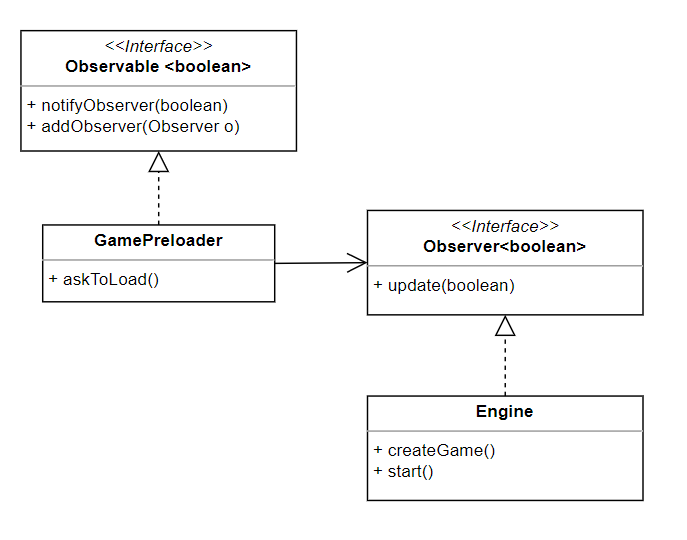
\includegraphics[width=\textwidth]{img/UML_ObserverRaffo.png}
	\caption{Schema UML architetturale del pattern Observer (Federico Raffoni).}
	\label{img:FedericoRaffoni_Observer}
\end{figure}

\subsection{Linda Fabbri}
La parte di progetto riguardo al design di cui mi sono occupata personalmente è quella riguardante i blocchi. 

Questa parte è composta da una classe enum (BlockType) per la classificazione delle tipologie dei vari blocchi, in base alla tipologia ho avuto la necessità di implementare metodi diversi, dunque ho creato tre interfacce: \textbf{Block} per tutti i generici blocchi, \textbf{FieldBlock} (estensione di Block) a cui ho aggiunto i metodi per i blocchi coltivabili (FIELD in BlockType), \textbf{UnlockableBlock}(estensione di FieldBlock) a cui ho aggiunto i metodi per i blocchi coltivabili bloccati (LOCKED in BlockType).

L’implementazione di queste interfacce si trova in FactoryBlock come classi innestate. Inoltre, per ogni tipologia di blocco si ha un differente costruttore al fine di determinare i vari campi. 

Ho scelto l’utilizzo del pattern \textit{“Factory method”} allo scopo di creare e ritornare blocchi in base al loro tipo mediante l’uso di costruttori differenti, delegando la responsabilità della scelta della creazione di ogni oggetto solo alla classe che implementa tale pattern.

In \Cref{img:LindaFabbri_Factory} è esemplificato il diagramma UML che descrive l'architettura Factory Method, mostrando le classi principali.

\hfill\break
\begin{figure}[!htb]
	\centering{}
	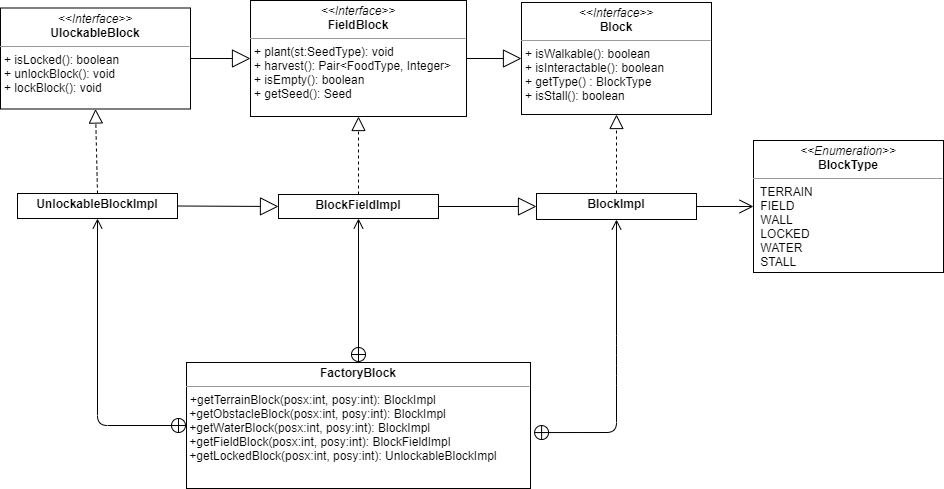
\includegraphics[width=\textwidth]{img/UML_FactoryLinda.png}
	\caption{Schema UML architetturale del pattern Factory Method (Linda Fabbri).}
	\label{img:LindaFabbri_Factory}
\end{figure}

\subsection{Giacomo Montali}

I principali punti dei quali mi sono occupato in questo progetto sono le varie entità presenti in essa, cioè il Player e i vari animali. 

In particolare per questi ultimi ho utilizzato il pattern \textit{“Simple Factory”}  nella classe \textbf{FactoryAnimal}, con l’obiettivo di delegare la creazione degli animali a quest’ultima, separandola così dalla classe \textbf{AnimalImpl}. La suddivisione degli animali è stata effetuata grazie ad Enum.

Inoltre ho creato la classe abstract \textbf{Entity} per renderla classe padre delle classi \textbf{PlayerImpl} e \textbf{AnimalImpl}, per evitare il riutilizzo di codice derivato dai metodi in comune come tutti i metodi che riguardano il movimento e la posizione sulla mappa.

In \Cref{img:GiacomoMontali_Abstract} è esemplificato il diagramma UML che descrive l'architettura delle classe Abstract Entity, mostrando le classi principali.

\hfill\break
\begin{figure}[!htb]
	\centering{}
	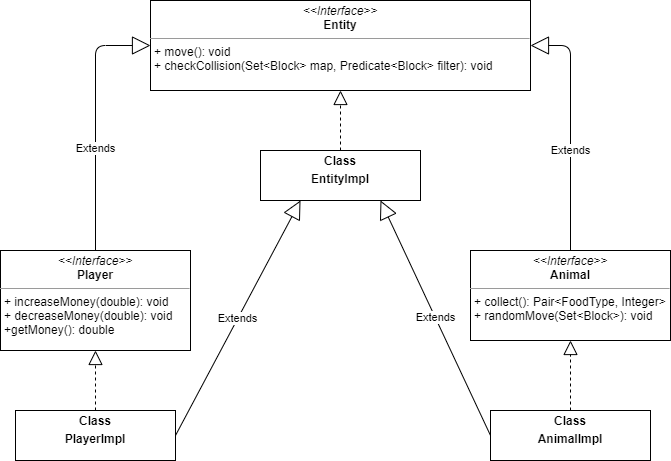
\includegraphics[width=\textwidth]{img/UML_AbstractMonta.png}
	\caption{Schema UML architetturale della clase Entity (Giacomo Montali).}
	\label{img:GiacomoMontali_Abstract}
\end{figure}

\chapter{Sviluppo}
\section{Testing automatizzato}


In questo progetto abbiamo deciso di testare prevalentemente la parte di Model poiché riteniamo sia la più propensa ad avere bug. Per svolgere test completamente automatizzati sul progetto è stato usato JUnit5.

Le classi che sono state testate sono:
\begin{itemize}
	\item \textbf{testPlayerMovement:} con questo test muovo il personaggio simulando la pressione dei tasti  
	\item \textbf{testPlayerCollision:} con questo test controllo che non avvenga il movimento su blocchi o in direzioni in cui mi è permesso
	\item \textbf{testPlayerPlant:} con questo test simulo l'interazione del personaggio con un blocco di tipo FieldBlock, piantando un seme e poi controllando che quel blocco non sia vuoto
	\item \textbf{testUnlockBlock:} con questo test simulo l'interazione con un blocco di tipo UnlockableBlock
	\item \textbf{testUnlockBlockWithoutMoney:} con questo test simulo l'interazione con un blocco di tipo UnlockableBlock senza soldi
	\item \textbf{testPlayerAnimalInteraction:} con questo test mi sposto nella zona "Stalla" della mappa e aspetto che un Animal qualunque sia pronto per poi poter raccogliere il suo \textit{Food} simulando l'interazione tra \textit{Player} e \textit{Animal}
	\item \textbf{testBuy:} con questo test provo a comprare un \textit{Seed} dallo \textit{Shop}, controllando poi che sia effettivamente presente nell'\textit{Inventory}
	\item \textbf{testBuyWithoutMoney:} questo test è simile al precedente, ma ho zero money, verificando che non avvenga l'acquisto
	\item \textbf{testSell:} in questo test simulo una normale interazione con un FieldBlock, ricavandone poi il raccolto che proverò a vendere, verificandone l'esistenza nell'inventario e l'ottenimento dei soldi ricavati dalla vendita
	\item \textbf{testSaver:} con questo test simulo il salvataggio del gioco su file con relativa apertura da esso in una nuova esecuzione del gioco, verificando che i nuovi e vecchi \textit{Game} e \textit{Player} siano gli stessi e abbiano le stesse caratteristiche
	\item \textbf{testSaverPlayer:} questo test è simile al precedente, differisce semplicemente per il fatto che il Player viene mosso nella nuova istanza di gioco, così da far risultare falso il fatto che l'istanza salvata e l'istanza nuova creata siano uguali

	
	
\end{itemize}




\section{Metodologia di lavoro}

Ci aspettiamo, leggendo questa sezione, di trovare conferma alla divisione operata nella sezione del design di dettaglio, e di capire come è stato svolto il lavoro di integrazione.
%
\textbf{Andrà realizzata una sotto-sezione separata per ciascuno studente} che identifichi le porzioni di progetto sviluppate, separando quelle svolte in autonomia da quelle sviluppate in collaborazione.
%
Diversamente dalla sezione di design, in questa è consentito elencare package/classi, se lo studente ritiene sia il modo più efficace di convogliare l'informazione.
%
Si ricorda che l'impegno deve giustificare circa 40-50 ore di sviluppo (è normale e fisiologico che approssimativamente la metà del tempo sia impiegata in analisi e progettazione).

\subsection*{Elementi positivi}

\begin{itemize}
	\item Si identifica con precisione il ruolo di ciascuno all'interno del gruppo, ossia su quale parte del progetto ciascuno dei componenti si è concentrato maggiormente.
	\item La divisione dei compiti è equa, ossia non vi sono membri del gruppo che hanno svolto molto più lavoro di altri.
	\item La divisione dei compiti è coerente con quanto descritto nelle parti precedenti della relazione.
	\item La divisione dei compiti è realistica, ossia le dipendenze fra le parti sviluppate sono minime.
	\item Si identifica quale parte del software è stato sviluppato da tutti i componenti insieme.
	\item Si spiega in che modo si sono integrate le parti di codice sviluppate separatamente, evidenziando eventuali problemi. Ad esempio, una strategia è convenire sulle interfacce da usare (ossia, occuparsi insieme di stabilire l'architettura) e quindi procedere indipendentemente allo sviluppo di parti differenti. Una possibile problematica potrebbe essere una dimenticanza in fase di design architetturale che ha costretto ad un cambio e a modifiche in fase di integrazione. Una situazione simile è la norma nell'ingegneria di un sistema software non banale, ed il processo di progettazione top-down con raffinamento successivo è il così detto processo ``a spirale''.
	\item Si descrive in che modo è stato impiegato il DVCS.
\end{itemize}

\subsection*{Elementi negativi}
\begin{itemize}
	\item Non si chiarisce chi ha fatto cosa.
	\item C'è discrepanza fra questa sezione e le sezioni che descrivono il design dettagliato.
	\item Tutto il progetto è stato svolto lavorando insieme invece che assegnando una parte a ciascuno.
	\item Non viene descritta la metodologia di integrazione delle parti sviluppate indipendentemente.
	\item Uso superficiale del DVCS.
\end{itemize}

\section{Note di sviluppo}

Questa sezione, come quella riguardante il design dettagliato va svolta \textbf{singolarmente da ogni membro del gruppo}.

Ciascuno dovrà mettere in evidenza eventuali particolarità del suo metodo di sviluppo, ed in particolare:
\begin{itemize}
	\item \textbf{Elencare} (fare un semplice elenco per punti, non un testo!) le feature \textit{avanzate} del linguaggio e dell'ecosistema Java che sono state
utilizzate. Le feature di interesse sono:
	\begin{itemize}
		\item Progettazione con generici, ad esempio costruzione di nuovi tipi generici, e uso di generici bounded. Uso di classi generiche di libreria non è considerato avanzato.
		\item Uso di lambda expressions
		\item Uso di \texttt{Stream}, di \texttt{Optional} o di altri costrutti funzionali
		\item Uso della reflection
		\item Definizione ed uso di nuove annotazioni
		\item Uso del Java Platform Module System
		\item Uso di parti di libreria non spiegate a lezione (networking, compressione, parsing XML, eccetera...)
		\item Uso di librerie di terze parti (incluso JavaFX): Google Guava, Apache Commons...
		\item Uso di build systems
	\end{itemize}
	Si faccia molta attenzione a non scrivere banalità, elencando qui features di tipo ``core'', come le eccezioni, le enumerazioni, o le inner class: nessuna di queste è considerata avanzata.
	\item Descrivere \textit{molto brevemente} le librerie utilizzate nella propria parte di progetto, se non trattate a lezione (ossia, se librerie di terze parti e/o se componenti del JDK non visti, come le socket). Si ricorda che l'utilizzo di librerie è valutato \emph{positivamente}.
	\item Sviluppo di algoritmi particolarmente interessanti \emph{non forniti da alcuna libreria} (spesso può convenirvi chiedere sul forum se ci sia una libreria per fare una certa cosa, prima di gettarvi a capofitto per scriverla voi stessi).
\end{itemize}
%
In questa sezione, \textit{dopo l'elenco}, è anche bene evidenziare eventuali pezzi di codice ``riadattati'' (o scopiazzati...) da Internet o da altri progetti, pratica che tolleriamo ma che non raccomandiamo.
%
I pattern di design, invece \textbf{non} vanno messi qui.
%
L'uso di pattern di design (come suggerisce il nome) è un aspetto avanzato di design, non di implementazione,
e non va in questa sezione.

\subsection*{Elementi positivi}

\begin{itemize}
	\item Si elencano gli aspetti avanzati di linguaggio che sono stati impiegati
	\item Si elencano le librerie che sono state utilizzate
	\item Si descrivono aspetti particolarmente complicati o rilevanti relativi all'implementazione,
ad esempio, in un'applicazione performance critical, un uso particolarmente avanzato di meccanismi
di caching, oppure l'implementazione di uno specifico algoritmo.
	\item Se si è utilizzato un particolare algoritmo, se ne cita la fonte originale. Ad esempio, se
si è usato Mersenne Twister per la generazione dei numeri pseudo-random, si cita \cite{mersenne}.
	\item Si identificano parti di codice prese da altri progetti, dal web, o comunque scritte in forma originale da altre persone. In tal senso, si ricorda che agli ingegneri non è richiesto di re-inventare la ruota continuamente: se si cita debitamente la sorgente è tollerato fare uso di di snippet di codice per risolvere velocemente problemi non banali. Nel caso in cui si usino snippet di codice di qualità discutibile, oltre a menzionarne l'autore originale si invitano gli studenti ad adeguare tali parti di codice agli standard e allo stile del progetto. Contestualmente, si fa presente che è largamente meglio fare uso di una libreria che copiarsi pezzi di codice: qualora vi sia scelta (e tipicamente c'è), si preferisca la prima via.
\end{itemize}

\subsection*{Elementi negativi}
\begin{itemize}
	\item Si elencano feature core del linguaggio invece di quelle segnalate. Esempi di feature
core da non menzionare sono:
    \begin{itemize}
        \item eccezioni;
        \item classi innestate;
        \item enumerazioni;
        \item interfacce.
    \end{itemize}
	\item Si elencano applicazioni di terze parti (peggio se per usarle occorre licenza, e lo
studente ne è sprovvisto) che non c'entrano nulla con lo sviluppo, ad esempio:
    \begin{itemize}
        \item Editor di grafica vettoriale come Inkscape o Adobe Illustrator;
        \item Editor di grafica scalare come GIMP o Adobe Photoshop;
        \item Editor di audio come Audacity;
        \item Strumenti di design dell'interfaccia grafica come SceneBuilder: il codice è in ogni caso inteso come sviluppato da voi.
    \end{itemize}
	\item Si descrivono aspetti di scarsa rilevanza, o si scende in dettagli inutili.
	\item Sono presenti parti di codice sviluppate originalmente da altri che non vengono
debitamente segnalate. In tal senso, si ricorda agli studenti che i docenti hanno accesso a tutti i
progetti degli anni passati, a Stack Overflow, ai principali blog di sviluppatori ed esperti Java (o sedicenti tali), ai blog dedicati allo sviluppo di soluzioni e applicazioni (inclusi blog dedicati ad Android e allo sviluppo di videogame), nonché ai social network. Conseguentemente, è \emph{molto} conveniente \emph{citare} una fonte ed usarla invece di tentare di spacciare per proprio il lavoro di altri.
	\item Si elencano design pattern
\end{itemize}

\chapter{Commenti finali}

In quest'ultimo capitolo si tirano le somme del lavoro svolto e si delineano eventuali sviluppi
futuri.

\textit{Nessuna delle informazioni incluse in questo capitolo verrà utilizzata per formulare la valutazione finale}, a meno che non sia assente o manchino delle sezioni obbligatorie.
%
Al fine di evitare pregiudizi involontari, l'intero capitolo verrà letto dai docenti solo dopo aver formulato la valutazione.

\section{Autovalutazione e lavori futuri}

\textbf{È richiesta una sezione per ciascun membro del gruppo, obbligatoriamente}.
%
Ciascuno dovrà autovalutare il proprio lavoro, elencando i punti di forza e di debolezza in quanto prodotto.
Si dovrà anche cercare di descrivere \emph{in modo quanto più obiettivo possibile} il proprio ruolo all'interno del gruppo.
Si ricorda, a tal proposito, che ciascuno studente è responsabile solo della propria sezione: non è un problema se ci sono opinioni contrastanti, a patto che rispecchino effettivamente l'opinione di chi le scrive.
Nel caso in cui si pensasse di portare avanti il progetto, ad esempio perché effettivamente impiegato, o perché sufficientemente ben riuscito da poter esser usato come dimostrazione di esser capaci progettisti, si descriva brevemente verso che direzione portarlo.

\section{Difficoltà incontrate e commenti per i docenti}

Questa sezione, \textbf{opzionale}, può essere utilizzata per segnalare ai docenti eventuali problemi o difficoltà incontrate nel corso o nello svolgimento del progetto, può essere vista come una seconda possibilità di valutare il corso (dopo quella offerta dalle rilevazioni della didattica) avendo anche conoscenza delle modalità e delle difficoltà collegate all'esame, cosa impossibile da fare usando le valutazioni in aula per ovvie ragioni.
%
È possibile che alcuni dei commenti forniti vengano utilizzati per migliorare il corso in futuro: sebbene non andrà a vostro beneficio, potreste fare un favore ai vostri futuri colleghi.
%
Ovviamente \textit{il contenuto della sezione non impatterà il voto finale}.

\appendix
\chapter{Guida utente}

Capitolo in cui si spiega come utilizzare il software. Nel caso in cui il suo uso sia del tutto
banale, tale capitolo può essere omesso.
%
A tal riguardo, si fa presente agli studenti che i docenti non hanno mai utilizzato il software
prima, per cui aspetti che sembrano del tutto banali a chi ha sviluppato l'applicazione possono non
esserlo per chi la usa per la prima volta.
%
Se, ad esempio, per cominciare una partita con un videogioco è necessario premere la barra
spaziatrice, o il tasto ``P'', è necessario che gli studenti lo segnalino.

\subsection*{Elementi positivi}

\begin{itemize}
 \item Si istruisce in modo semplice l'utente sull'uso dell'applicazione, eventualmente facendo uso di schermate e descrizioni.
\end{itemize}

\subsection*{Elementi negativi}
\begin{itemize}
 \item Si descrivono in modo eccessivamente minuzioso tutte le caratteristiche, anche minori, del software in oggetto.
 \item Manca una descrizione che consenta ad un utente qualunque di utilizzare almeno le funzionalità primarie dell'applicativo.
\end{itemize}

\chapter{Esercitazioni di laboratorio}

In questo capitolo ciascuno studente elenca gli esercizi di laboratorio che ha svolto
(se ne ha svolti),
elencando i permalink dei post sul forum dove è avvenuta la consegna.

\section*{Esempio}

\subsection{Paolino Paperino}

\begin{itemize}
 \item Laboratorio 04: \url{https://virtuale.unibo.it/mod/forum/discuss.php?d=12345#p123456}
 \item Laboratorio 06: \url{https://virtuale.unibo.it/mod/forum/discuss.php?d=22222#p222222}
 \item Laboratorio 09: \url{https://virtuale.unibo.it/mod/forum/discuss.php?d=99999#p999999}
\end{itemize}

\subsection{Paperon De Paperoni}

\begin{itemize}
 \item Laboratorio 04: \url{https://virtuale.unibo.it/mod/forum/discuss.php?d=12345#p123456}
 \item Laboratorio 05: \url{https://virtuale.unibo.it/mod/forum/discuss.php?d=22222#p222222}
 \item Laboratorio 06: \url{https://virtuale.unibo.it/mod/forum/discuss.php?d=99999#p999999}
 \item Laboratorio 07: \url{https://virtuale.unibo.it/mod/forum/discuss.php?d=22222#p222222}
 \item Laboratorio 08: \url{https://virtuale.unibo.it/mod/forum/discuss.php?d=99999#p999999}
 \item Laboratorio 09: \url{https://virtuale.unibo.it/mod/forum/discuss.php?d=22222#p222222}
 \item Laboratorio 10: \url{https://virtuale.unibo.it/mod/forum/discuss.php?d=99999#p999999}
 \item Laboratorio 11: \url{https://virtuale.unibo.it/mod/forum/discuss.php?d=22222#p222222}
\end{itemize}


\bibliographystyle{alpha}
\bibliography{13-template}

\end{document}
